\appendix


\section{Listing of the Complete Probability Density Functions}\label{sec:ResFit:App:Pdf}

In the following, the complete dijet pdfs are listed, including the normalisation.

The simplified pdf~\qeq{eq:ResFit::DijetPdfTransformed:Simple} of the asymmetry with \mbox{$f(\pttrue)  = \delta\left(\pttrue - \ptave\right)$} is given by
\begin{align}
  \begin{split}
    \label{eq:ResFit:App:SimplePdf}
    g_{\sigma'}\left(\Delta\pt\right) & = \frac{1}{\mathcal{N}}\cdot\left\{
      \begin{array}{rl}
        \exp\left[-\frac{1}{2}\left(\frac{\Delta\pt}{\sigma'}\right)^{2}\right] & \quad\text{for } |\Delta\pt| < |\Delta\pt|_{\text{max}} \\
        & \\
        0 & \quad\text{otherwise}
      \end{array}
    \right. \;, \\
    \mathcal{N} & = \sqrt{2\pi}\sigma'\text{erf}\left(\frac{\Delta\pt}{\sqrt{2}\sigma'}\right) \;.
  \end{split}
\end{align}  

The full pdf~\qeq{eq:ResFit:DijetPdfTransformed} including the spectrum~\qeq{eq:ResFit:DataDriven:ModifiedSpectrum} is given by
\begin{align}
  \begin{split}
    \label{eq:ResFit:App:FullPdf}
    g_{\sigma'}\left(\ptave,\Delta\pt\right) & =
    \frac{1}{\mathcal{N}}\cdot\left\{
      \begin{array}{rl}
        \exp\left[-\frac{1}{2}\left(\frac{\Delta\pt}{\sigma'}\right)^{2}\right]\cdot\int\dif{\pttrue}\bigg\{f_{0}\left(\pttrue\right)\Big[\text{erf}\left(\frac{\ptavemax-\pttrue}{\sqrt{2}\sigma'}\right)  & \quad\text{for } |\Delta\pt| < |\Delta\pt|_{\text{max}}\text{ and} \\
        - \text{erf}\left(\frac{\ptavemin-\pttrue}{\sqrt{2}\sigma'}\right)\Big]\exp\left[-\frac{1}{2}\left(\frac{\ptave - \pttrue}{\sigma'}\right)^{2}\right]\bigg\} & \quad\ptavemin < \ptave < \ptavemax \\
        & \\
        0 & \quad\text{otherwise}
      \end{array}
    \right. \;, \\
    \mathcal{N} & = \pi\sigma'^{2}\text{erf}\left(\frac{\Delta\pt}{\sqrt{2}\sigma'}\right)\int\dif{\pttrue}\;f_{0}\left(\pttrue\right)\left[\text{erf}\left(\frac{\ptavemax-\pttrue}{\sqrt{2}\sigma'}\right) - \text{erf}\left(\frac{\ptavemin-\pttrue}{\sqrt{2}\sigma'}\right)\right]^{2}
    \;.
  \end{split}
\end{align}



\section{Determination of the Gaussian MC Truth Resolution}\label{sec:ResFit:App:MCTruth}

The resolution of the simulated jets, derived from MC truth information, is used as a reference in the closure tests of the maximum likelihood method.
For its determination, the same MC sample and corrected jets as before (comp. \qsec{sec:ResFit:EvtSel}) have
been used, however none of the additional selection, \eg the requirement
on $|\Delta\phi_{i}|$, has been performed.
Also, events have not been weighted to the realisitic QCD spectrum but
rather the actual generated number of events has been used in order
to achieve roughly the same statistical precision over the whole \pt range.

\begin{figure}[ht]
  \centering
  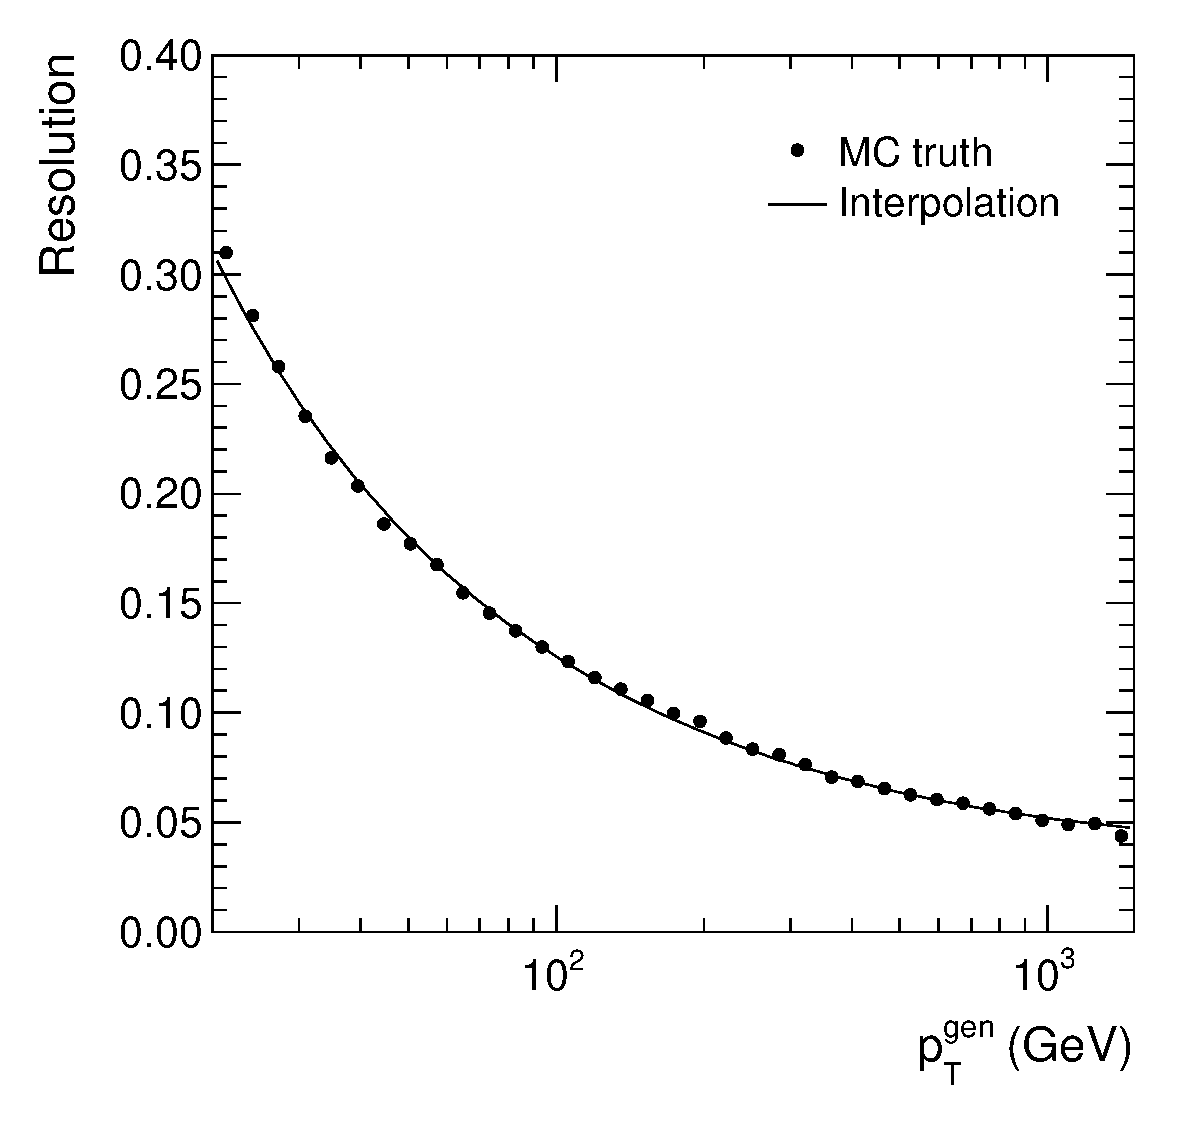
\includegraphics[width=0.45\textwidth]{figures/hMCTruthReso}
  \caption{MC truth resolution for \mbox{$|\eta| < 1.3$}.
  The widths (circles) of Gaussian fits to the response distributions
  \mbox{$\pt/\ptgen$} in different \ptgen bins are interpolated with the
  smooth function~\qeq{eq:ResFit:MCTruthReso} (solid line).}
  \label{fig:ResFit:App:MCTruthReso}
\end{figure}

For each event, the two particle level jets with the highest \ptgen
are selected and the detector level jet closest in
\mbox{$\Delta R = \sqrt{(\Delta\eta)^{2} + (\Delta\phi)^{2}}$} is assigned to each.
The event is discarded if for one of the pairs $\Delta R > 0.2$.
Then, for different bins of \ptgen and $\eta$, the response $\pt/\ptgen$ of each pair is filled into a
histogram and the bulk of the distribution, defined by the interval of
$1.5$ standard deviations around the mean, is fitted with a Gaussian.
The widths $\sigma_{\text{MC}}$ of the fitted Gaussians in different \ptgen
bins are shown in \qfig{fig:ResFit:App:MCTruthReso} for \mbox{$|\eta| < 1.3$}.
They are interpolated with the function
\begin{equation}
  \label{eq:ResFit:MCTruthReso}
  \sigma_{MC}(\ptgen) = \frac{a_{1}}{\ptgen/\gev} \oplus
  \frac{a_{2}}{\sqrt{\pt/\gev}} \oplus a_{3} \; ,
\end{equation}
which has been used as MC truth resolution throughout this note.
The fitted parameter values are listed in \qtab{tab:ResFit:MCTruthReso}.

\begin{table}[ht]
  \caption{Parameter values of the MC truth resolution \qeq{eq:ResFit:MCTruthReso}.
    The uncertainties assigned to the fitted values are the
    statistical uncertainties from the interpolation.}
  \centering
  \begin{tabular}[ht]{ccccc}
    \toprule
    $|\eta_{\text{min}}|$ & $|\eta_{\text{max}}|$ & $a_{1}$ & $a_{2}$ & $a_{3}$ \\
    \midrule
    $0$ & $1.3$ & $3.044 \pm 0.069$ & $1.1601 \pm 0.0056$ & $0.03482 \pm 0.00046$ \\
   \bottomrule
  \end{tabular}
  \label{tab:ResFit:MCTruthReso}
\end{table}



\section{Study with a Toy Monte Carlo Simulation}\label{sec:ResFit:App:ToyMC}

A very basic closure test of the maximum likelihood fit has been performed using a toy MC simulation.

A sample of $30\,000$ ideal dijet events has been generated assuming a simple exponential particle level jet \pt spectrum
\begin{equation}
  \label{eq:ResFit:ToyMC:Spectrum}
  f\left(\pttrue\right) \propto \exp\left(-\pttrue / \tau\right),
  \qquad \tau = 80 \;,
\end{equation}
ranging from \mbox{$50 < \pttrue < 1\,000\gev$} (comp. \qfig{fig:ResFit:App:ToyMC:Spectrum}).
Two independent measurements of the jet \pt have been simulated by weighting \pttrue with random numbers according to a Gaussian response pdf \mbox{$r_{\mathbf{\xi}}(\pt|\pttrue) = \mathcal{G}(\pt;\pttrue,\sigma)$}.
The standard deviation, \ie the jet resolution, $\sigma$ has been parametrised as a function of \pttrue and the parameters $\xi_{j}$, \mbox{$j\in [1,3]$}, as
\begin{equation}
  \label{eq:ResFit:ToyMC:Sigma}
  \sigma_{\xi_{j}}\left(\pt\right) = \xi_{1}\gev \oplus \xi_{2}\,\sqrt{\pt\gev}\oplus \xi_{3}\pt \;;
\end{equation}
the values of the parameters $\xi_{j}$ are listed in \qtab{tab:ResFit:ToyMC:FitResult}.
Examples of simulated response distributions are shown in \qfig{fig:ResFit:App:ToyMC:Response} for two different \pttrue bins.

\begin{figure}[ht]
  \centering
  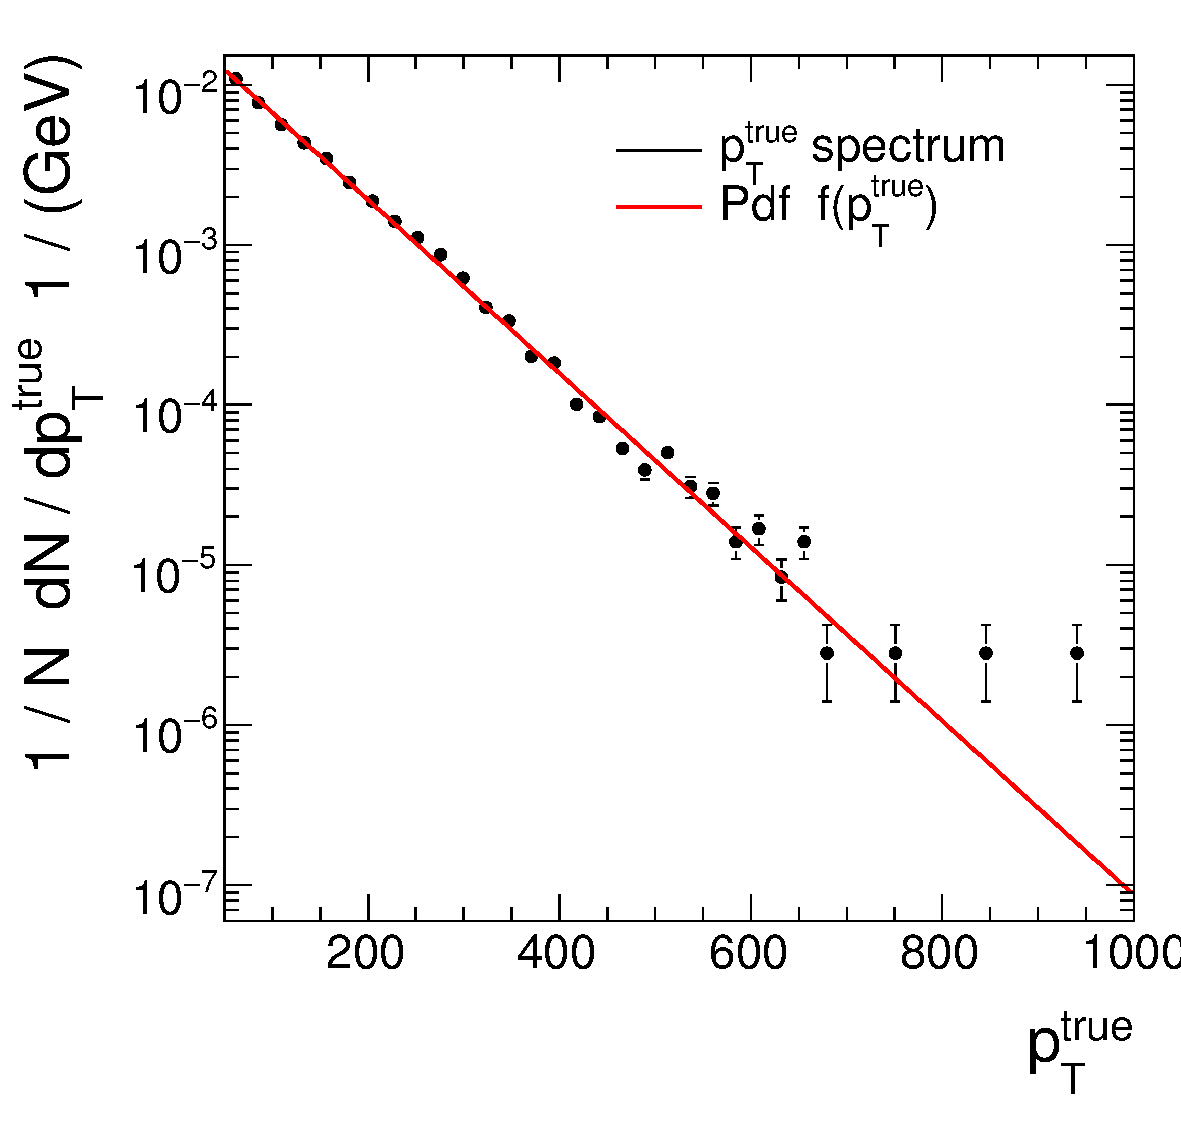
\includegraphics[width=0.45\textwidth]{figures/resFit_ToyMC_PtGenCuts_SpectrumLog}
  \caption{Toy Monte Carlo simulation of a sample of ideal dijet events.
    Generated \pttrue spectrum (circles) and the underlying pdf (solid line).}
  \label{fig:ResFit:App:ToyMC:Spectrum}
\end{figure}

\begin{table}[ht]
  \caption{Parameter values of the Gaussian jet \pt resolution $\sigma$.
    Listed are the true values used for the generation and the fitted values.
    The uncertainties assigned to the fitted values are the statistical uncertainties from the fit.
    \fixme{List global correlation coefficients.}}
  \centering
  \begin{tabular}[ht]{lccc}
    \toprule
     & $\xi_{1}$ & $\xi_{2}$ & $\xi_{3}$ \\
    \midrule
    True value & $4$           & $1.2$           & $0.05$ \\
    Fit result & $4.5 \pm 0.7$ & $1.18 \pm 0.05$ & $0.051 \pm 0.004$ \\
    \bottomrule
  \end{tabular}
  \label{tab:ResFit:ToyMC:FitResult}
\end{table}

\begin{figure}[ht]
  \centering
  \begin{tabular}{cc}
    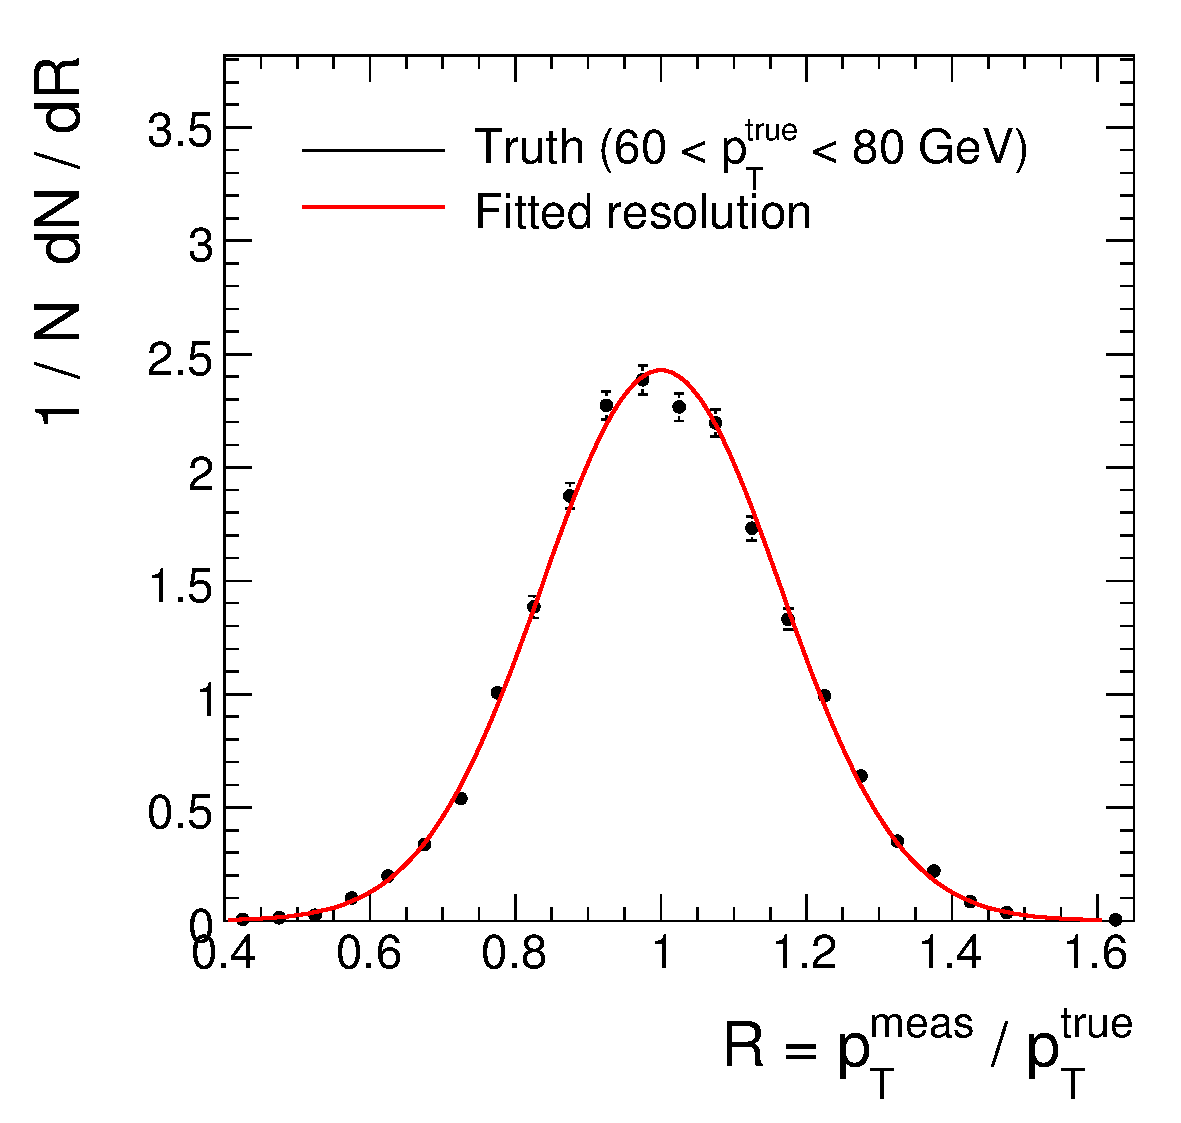
\includegraphics[width=0.45\textwidth]{figures/resFit_ToyMC_PtGenCuts_ResolutionBin1} &
    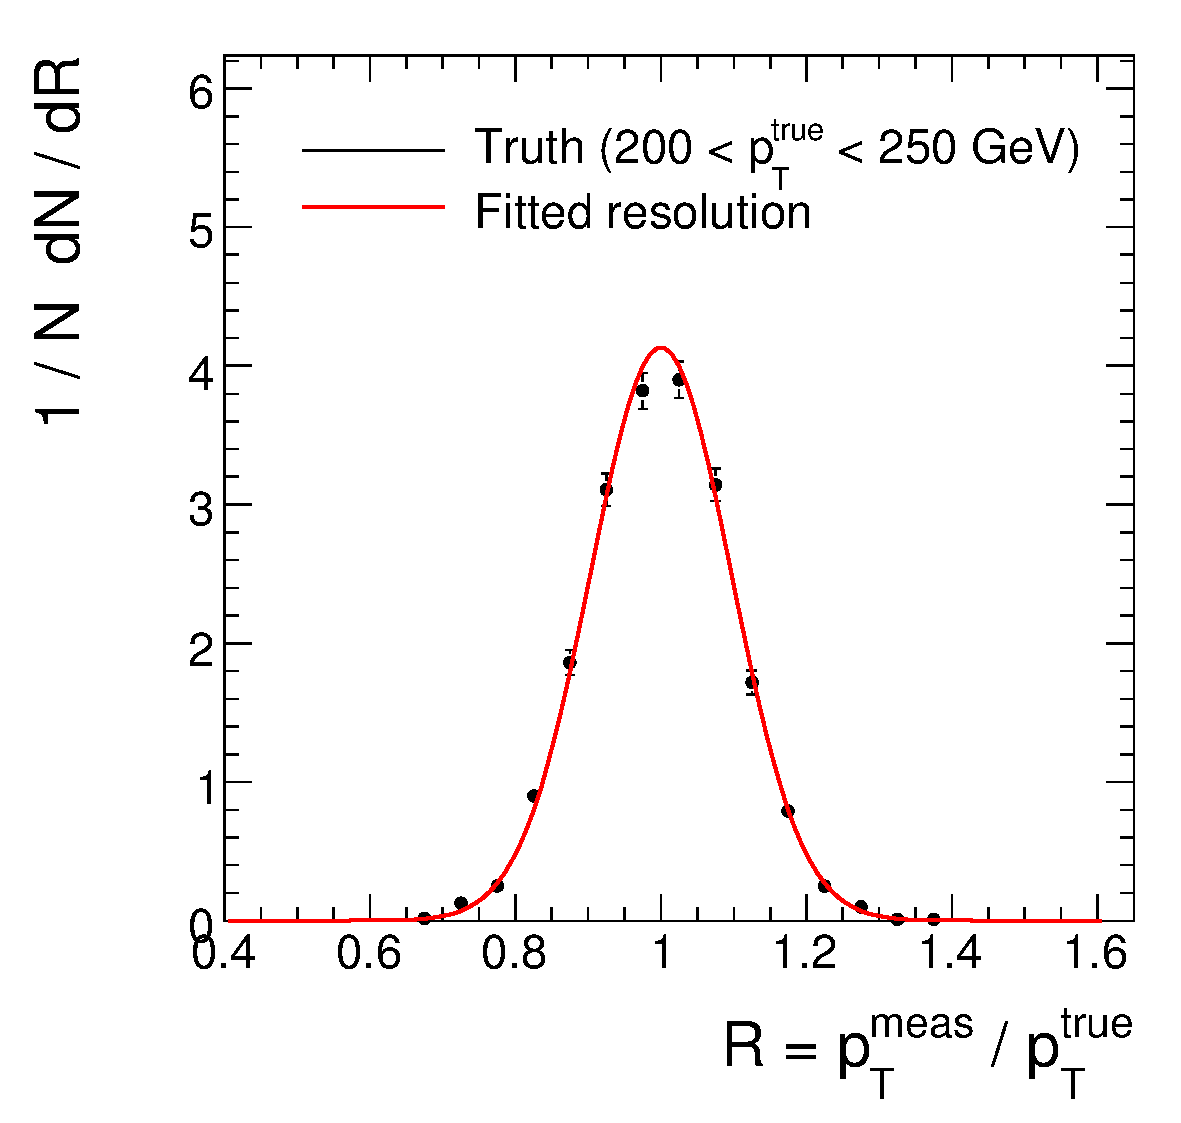
\includegraphics[width=0.45\textwidth]{figures/resFit_ToyMC_PtGenCuts_ResolutionBin7} \\      
  \end{tabular}
  \caption{Generated true response \mbox{$\pt / \pttrue$} (circles) and the response (solid line) from the maximum likelihood fit in two different \pttrue bins.
    The latter has been evaluated for the mean \pttrue in these bins.
    Note, here ``fit'' does not refer to a fit to the shown histogram but the maximisation of the likelihood~\eqref{eq:ResFit:Likelihood}.
  }
  \label{fig:ResFit:App:ToyMC:Response}
\end{figure}

\begin{figure}[ht]
  \centering
  \begin{tabular}{cc}
    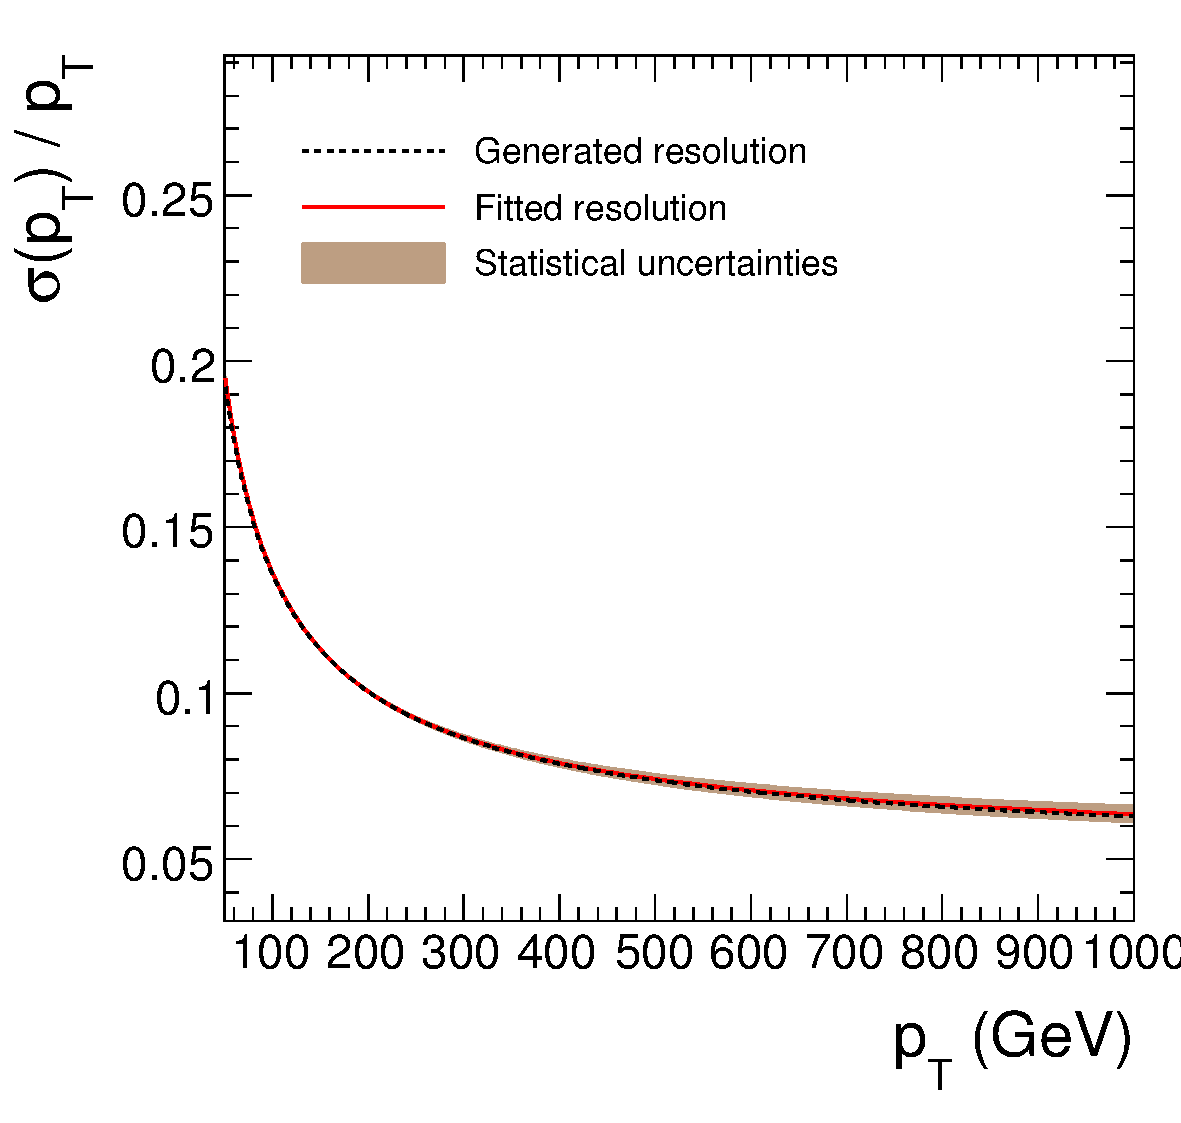
\includegraphics[width=0.45\textwidth]{figures/resFit_ToyMC_PtGenCuts_Sigma} &
    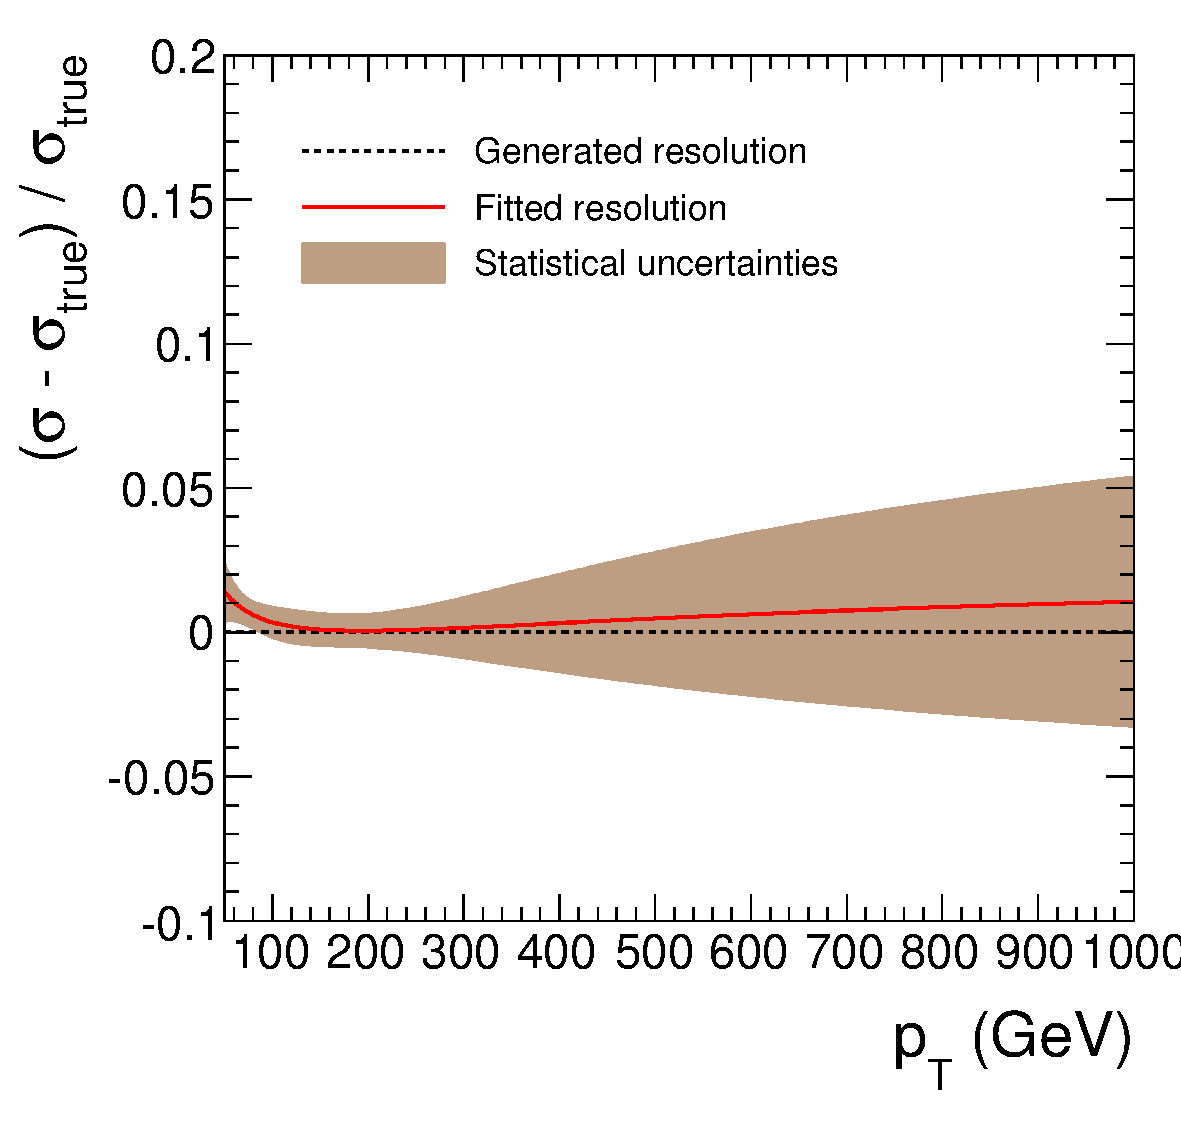
\includegraphics[width=0.45\textwidth]{figures/resFit_ToyMC_PtGenCuts_SigmaRelDifference} \\
  \end{tabular}
  \caption{(\textit{Left}) Relative Gaussian resolution \mbox{$\sigma(\pt)/\pt$} evaluated with the fitted parameter values (solid line) in comparison to the true resolution (dashed line) and (\textit{right}) the relative difference \mbox{$\sigma_{\text{fit}} / \sigma_{\text{true}}$}.
    The shaded areas represent the propagated statistical uncertainty on the fitted parameter values, taking into account the parameter correlations.}
  \label{fig:ResFit:App:ToyMC:FittedSigma}
\end{figure}

The jet \pt resolution is measured in this sample by maximisation of the dijet likelihood~\qeq{eq:ResFit:Likelihood}.
The jet \pt spectrum is taken directly from the simulation~\qeq{eq:ResFit:ToyMC:Spectrum}, whereupon the response is assumed to be Gaussian and the resolution $\sigma$ to depend on \pttrue as in~\qeq{eq:ResFit:ToyMC:Sigma}.
In difference to the procedure in data, \mbox{$\sigma = \sigma_{\xi_{j}}(\pttrue)$} is thus a \pttrue dependent function and the fitted parameters are the $\xi_{j}$.
Before, a \pt independent mean $\sigma$ has been fitted in bins of \ptave, which was necessary in order to extrapolate to the two jet only event topology and correct for the bias from additional jet activity (comp. \qsec{sec:ResFit:DataDriven:AddJets:Extrapolation}).
The fitted parameter values $\xi_{j}$ are listed in \qtab{tab:ResFit:ToyMC:FitResult}; they agree with the true values within the statistical uncertainties.
An example of the resulting response distribution in comparison to the true distribution is shown in \qfig{fig:ResFit:App:ToyMC:Response} for two different \pttrue bins.

The Gaussian resolution $\sigma_{\xi_{j}}(\pt)/\pt$, evaluated with the fitted parameter values $\xi_{j}$, is shown in \qfig{fig:ResFit:App:ToyMC:FittedSigma} in comparison to the true width at generation.
There is good agreement.
For \pt up to $\approx 600\gev$, where there is sufficient statistics in the generated sample (comp. \qfig{fig:ResFit:App:ToyMC:Spectrum}), the uncertainties are about $1\%$ at low \pt rising to about $3\%$.
For larger \pt the uncertainties rise up to $4.5\%$.


\clearpage